% !TeX spellcheck = en_GB
%%%%%%%%%%%%%%%%%%%%%%%%%% phdsymp_sample2e.tex %%%%%%%%%%%%%%%%%%%%%%%%%%%%%%
%% changes for phdsymp.cls marked with !PN
%% except all occ. of phdsymp.sty changed phdsymp.cls
%%%%%%%%%%              %%%%%%%%%%%%%
%%%%%%%%%% More information: see the header of phdsymp.cls %%%%%%%%%%%%%
%%%%%%%%%%              %%%%%%%%%%%%%
%%%%%%%%%%%%%%%%%%%%%%%%%%%%%%%%%%%%%%%%%%%%%%%%%%%%%%%%%%%%%%%%%%%%%%%%%%%%%%%


%\documentclass[10pt]{phdsymp} %!PN
\documentclass[twocolumn]{phdsymp} %!PN
%\documentclass[12pt,draft]{phdsymp} %!PN
%\documentstyle[twocolumn]{phdsymp}
%\documentstyle[12pt,twoside,draft]{phdsymp}
%\documentstyle[9pt,twocolumn,technote,twoside]{phdsymp}

\usepackage[english]{babel}  % Voor nederlandstalige hyphenatie (woordsplitsing)

\usepackage{graphicx}     % Om figuren te kunnen verwerken
\usepackage{graphics}			% Om figuren te verwerken.

\graphicspath{images/}

\PassOptionsToPackage{hyphens}{url}
\usepackage{url}

\usepackage[T1]{fontenc}

\hyphenation{}

\def\BibTeX{{\rm B\kern-.05em{\sc i\kern-.025em b}\kern-.08em
 T\kern-.1667em\lower.7ex\hbox{E}\kern-.125emX}}

\newtheorem{theorem}{Theorem}

\begin{document}

\title{The user perceived performance of route planning APIs} %!PN

\author{Bert Marcelis}

\supervisor{Prof. dr. ir. Ruben Verborgh, dr. ing. Pieter Colpaert, Julian Andres Rojas Melendez}

\maketitle

\begin{abstract}
For the Web architectures behind route planning applications, remote procedure calls are commonplace, in which a server calculates the routes for all end-users. Linked Connections introduces an alternative architecture following the \textsc{rest} constraints, publishing the raw data in fragments. While benchmarks show a higher cost-efficiency of Linked Connections on the server, it is currently not known how it performs on clients, that now also need to execute the route planning algorithm. In this work, we study the user-perceived performance of route planning on the client-side, consuming more bandwidth, versus route planning on the server-side. An isomorphic app was developed with both route planning on the client-side as on the server-side. Both technical performance and user-perceived performance were tested among 17 travellers, and 81 respondents gave insights on their use of travel companions.
We found that the performance of the client-side Android Linked Connections implementation heavily depends on the type of information, the query and the user’s device. Linked Connections can be faster or slower than a query answering \textsc{api} based on these parameters. For a majority of the users, the benefit of off-line searches outweighs the slower speed of Linked Connections and even though Linked Connections is slower than the reference \textsc{api}, users consider it as fast as their default application on recent devices.


\end{abstract}

\begin{keywords}
Linked Connections, public transport, linked data, web engineering
\end{keywords}

\section{Introduction}
\PARstart{P}{ublic} transport is an essential aspect of modern cities. To make use of it, travellers frequently use their smartphones (applications) or public transport companies' websites to get route planning advice. Today most of these mobile and Web applications follow a client-server architecture that makes use of Remote Procedure Call (\textsc{rpc}) \textsc{api}s for exchanging data. In order to handle high volumes of requests, such an approach requires high levels of investment on computational infrastructure and also depends on a continuous connection between the client and the route planning server to answer any given query. A different approach consists on providing clients with all the necessary data of a given public transport network for them to be able to answer any query by themselves. This can be done by using the General Transport Format Specification (\textsc{gtfs}) and can be particularly useful when queries in bulk are needed, for example in insights building and analytics collecting applications. However this approach requires too much time and processing power to be applied in mobile end user devices.

Linked Connections emerges as an alternative approach that follows the \textsc{rest} constraints and consists on publishing the raw data in fragments, sorted in a timely fashion. Clients can download these data fragments and perform route-planning algorithms on top of them. Previous research has proven Linked Connections to be 75\% more cost-efficient~\cite{colpaert17} than \textsc{rpc}-based approaches. However, while performance and costs on server-side have been researched, the performance and user-experience for a client implementing Linked Connections are still unknown. In this work we explore various aspects of the performance and user-experience of a client-side Linked Connections-based application through the development of an isomorphic mobile application that compares the Linked Connections approach to a reference \textsc{rpc} \textsc{api}, which uses the same data and algorithms, but runs all calculations on server-side.

The remainder of this article is structured as follows. We first describe the state of the art. We then describe the meaning of user-perceived performance on Web architectures. Afterwards we describe the evaluation setup and the design choices. Then we present the results obtained and we finally present the discussion and conclusions drawn from this work.

\section{State of the art}
Applications for public transport are, at this time, commonly driven by \textsc{rpc} \textsc{api}s. These \textsc{api}s are based on dumb clients asking a smart server for an answer. On one hand this means it can be used on all kinds of clients, as it does not require much resources client-side to offer good performance~\cite{rpc}. On the other hand it can be costly, as every response is personalized, meaning the server has to do processor-intensive tasks for every query and needs to be scaled according to this load. Other negative aspects, specific for route planning, are the requirements for a constant internet connection, and the fact that individual developers can’t alter the route planning algorithm for their application. An \textsc{rpc} \textsc{api} can transfer data in various formats, for example using Simple Object Access Protocol (\textsc{soap}), \textsc{json} \textsc{rpc} or Representational State Transfer (\textsc{rest}). 

When transport data is needed in bulk, for example when someone wants to gather statistics, \textsc{gtfs}  can be used. \textsc{gtfs}  is divided into two categories, General Transit Format Specifications Static (\textsc{gtfs}) and General Transit Format Specifications Realtime (\textsc{gtfs-rt}). A \textsc{gtfs}  feed is composed of a series of text files collected in a ZIP file. Each file models a particular aspect of transit information: stops, routes, trips, and other schedule data\footnote{\textsc{gtfs} \url{https://developers.google.com/transit/gtfs/}}. Theses files link together in a similar fashion to a relational database. \textsc{gtfs}  Realtime is a feed specification that allows public transportation agencies to provide realtime updates about their fleet to application developers. It is an extension to \textsc{gtfs} ~\footnote{\textsc{gtfs-rt} \url{https://developers.google.com/transit/gtfs-realtime/}}, and is not of much use on its own.
While it is a resource-intensive task to deduce information from \textsc{gtfs} , it does not need \textsc{api} calls for every query. Unfortunately, due to \textsc{gtfs}  being resource intensive, it’s not fit for mobile devices or cases where results are needed quickly.

Linked connections tries to find a balance between these two technologies, by publishing the raw data in chronological, easy-to-use linked fragments. It’s proven to be server efficient, and when load increases, performance increases instead of decreases ~\cite{colpaert17}.

Both Linked Connections and \textsc{gtfs} require the implementation of a route planning algorithm in order to determine a route from A to B when needed. Route planning algorithms have been studied extensively in the past 50 years. Many algorithms solve this problem by using a graph, for example the Dijkstra algorithm~\cite{dijkstra} and the algorithm of Bellman-Ford~\cite{bellmanford}. These algorithms rely on a graph, modelled using neighbour-matrices or neighbour-lists. The Connection Scan Algorithm (\textsc{csa}) does not rely on these matrices or lists, but requires a chronological list of all vehicle departures~\cite{csa}. This makes \textsc{csa} perfectly fit for Linked Connections.

\section{User perceived performance of web architectures}
Every Web architecture has specific properties (e.g. latency, performance, cache reuse, etc)~\cite{verborgh16}. While these are all technical values, there is also the user-perceived performance, which is a subjective user experience. First defined by Roy T. Fielding~\cite{fielding99} as the latency between steady-states for a browser-based application, it comprises all processing needed, not only network traffic related. For a browser application, the total latency consists of the following parts:
\begin{enumerate}
	\item The time needed for the user agent to recognize the event that initiated the action
	\item The time required to set-up any interaction(s) between components
	\item The time required to transmit each interaction to the components
	\item The time required to process each interaction on those components
	\item The time required to complete sufficient transfer before the user agent is able to begin rendering a usable result.
	\item The time required to complete processing of the result of the interaction(s) before the user agent is able to begin rendering a usable result.
\end{enumerate}

While only steps 3, 4 and 5 are directly dependent on network connectivity, all of these steps can be influenced by the used architecture. When not only focussing on performance, but also on the way users interact with technology, it is important to define the user-experience (UX). \textsc{ux} is a broad term, originally designating the design and usage of interfaces, making it a synonym for interactions and usability. But it is also used for non-instrumental needs and experiences in a more complex way~\cite{avila11}. In this work \textsc{ux} will always be considered in this broader way.

\section{Evaluation design}

In order to evaluate Linked Connections and compare it to \textsc{rpc} \textsc{api}s, an isomorphic application was developed. This application allows to test the client-side Android route planning implementation and an \textsc{rpc} \textsc{api}, while keeping the user interface and client-side logic identical. The \textsc{rpc} \textsc{api}, \textsc{lc2irail}, is backed by the same data and algorithms as the client-side Linked Connections implementation, thus allowing a fair comparison. As a result, the only difference is which entity does the processing, and how data is exchanged.

Through this application, user testing was conducted on 17 test persons. Each tester was asked to search for data he/she usually searches for, one time using the reference \textsc{rpc} \textsc{api} as data provider, and using the client-side Android Linked Connections implementation the second time. After testing and grading the client-side Android Linked Connections implementation, they were also encouraged to turn off their network connection and test the off-line capabilities using Linked Connections. Users were only informed about the differences between both implementations after the test was completed, to prevent any type of bias on them. For each implementation, the user graded the listing speed of departures and arrivals for a station (liveboards), journeys from A to B (routes) and vehicle trips (vehicles). Users were also asked to compare each implementation to the application they usually use. To conclude, they had to explicitly choose between both implementations regarding speed for each endpoint, and which implementation they favoured the most, taking into account both speed and offline access.

In order to assess which aspects were more important to users, a survey was held for 81 travellers. This survey asked about past experiences, needs, mobile data, privacy, and concluded by shortly polling how interested respondents were in the features offered by Linked Connections.

Along with subjective experiences from users, objective benchmarks were also executed. These benchmarks used a fraction of the real-world searches handled by the iRail \textsc{api}\footnote{The iRail project: \url{https://hello.irail.be}}, to determine the speed needed to load a certain number of results. This was done both on a relatively modern smartphone (HTC 10, Android 8.0) and on an older smartphone (HTC One, Android 5.0). By running each benchmark on both devices, it was possible to evaluate the impact of the hardware on the client-side Linked Connections implementation.

For the local implementation, two versions were implemented. The first implementation relies on the default Android \textsc{json} parser, \emph{org.json}. This implementation proved to be rather slow, with vehicle requests taking around four seconds on the HTC 10. It used an index containing the first departure of every vehicle and it did not use a cache. CPU profiling for this implementation revealed heavy CPU usage by the \textsc{json} parsing process, for which several optimizations were applied. These optimizations proved to be insufficient, which is why a second implementation was built. This new implementation makes use of the \emph{LoganSquare} parser, resulting in a reduction of around one second for the same queries. Both implementations are available online\footnote{\url{https://github.com/Bertware/masterthesis-LC-LC2Irail-android-client/releases/tag/RESEARCH40}}.

\section{Results}

When testing both parsers with a cache memory on the device’s flash storage, performance increased even more, going from around four seconds to just below two seconds. Based on this, the user-test was altered. While the first ten users tested the first implementation, the last seven testers received the second implementation. The second group reported slightly faster experiences for routes and vehicles, but the separate test groups are too small to generalize this to the entire population. Users who tested both implementations reported an perceived speed gain, independent of the test device hardware. All benchmarks use the second (more efficient) implementation. Raw results are available online\footnote{\url{https://github.com/Bertware/masterthesis/blob/master/data.ods?raw=true}}.


\begin{figure}[ht]
	\begin{center}
		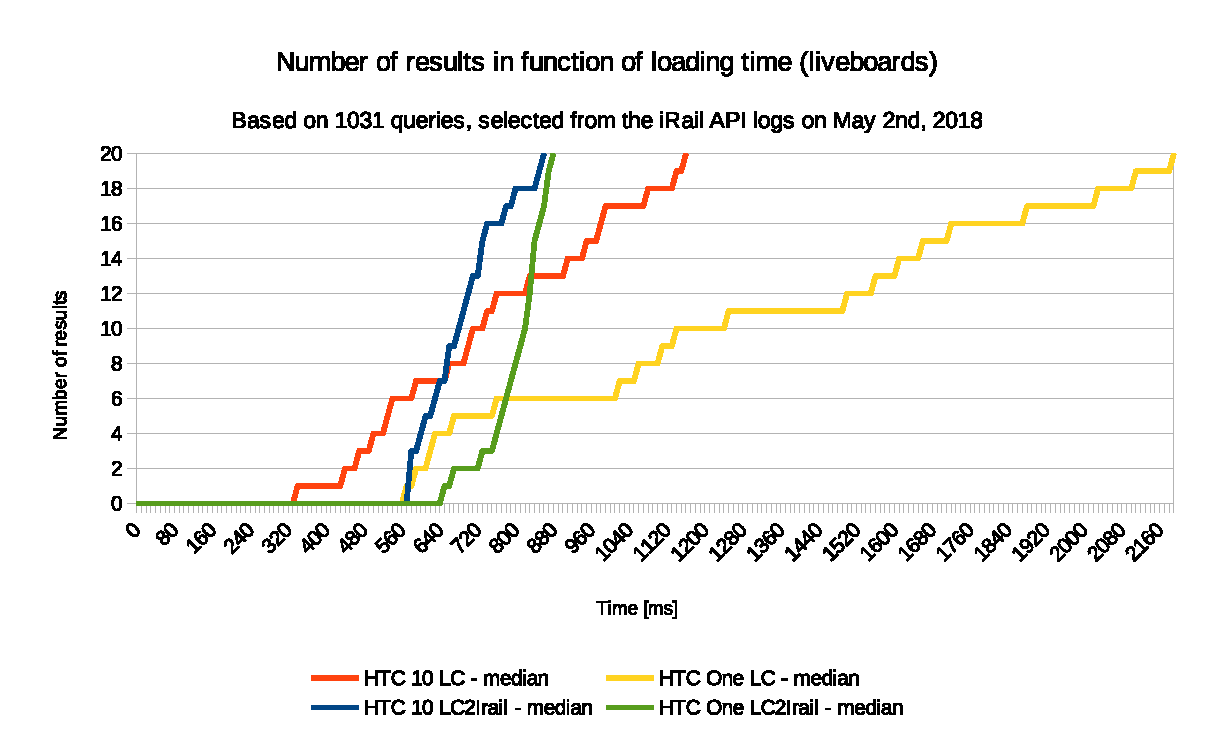
\includegraphics[width=.50\textwidth]{images/dief_liveboards_average.eps}
		\caption{\label{fig:liveboard} The median performance of loading incremental liveboard results using different Web architectures and different devices shows that for fast devices (HTC-10 LC) client-side filtering gives the first results faster than the serverside implementation (HTC-10 LC2IRAIL). This effect is also visible, yet less apparent, for the slower device (HTC One).}
	\end{center}
\end{figure}

The incremental results for liveboards shown in figure~\ref{fig:liveboard}, make clear that there are differences between both architectures. Linked Connections is faster than \textsc{lc2irail} (the reference \textsc{rpc} \textsc{api}) on both devices for the first few results. However, when ten results are needed – about the number of results which fit on a large screen – \textsc{lc2irail} is faster on both devices. It is clear that the \textsc{rpc} \textsc{api} performs similarly on both devices, but the Linked Connections client does not. There is a gap between the time needed by the client-side Linked Connections implementation on both devices, which grows with the number of results needed.

\begin{figure}[ht]
	\begin{center}
		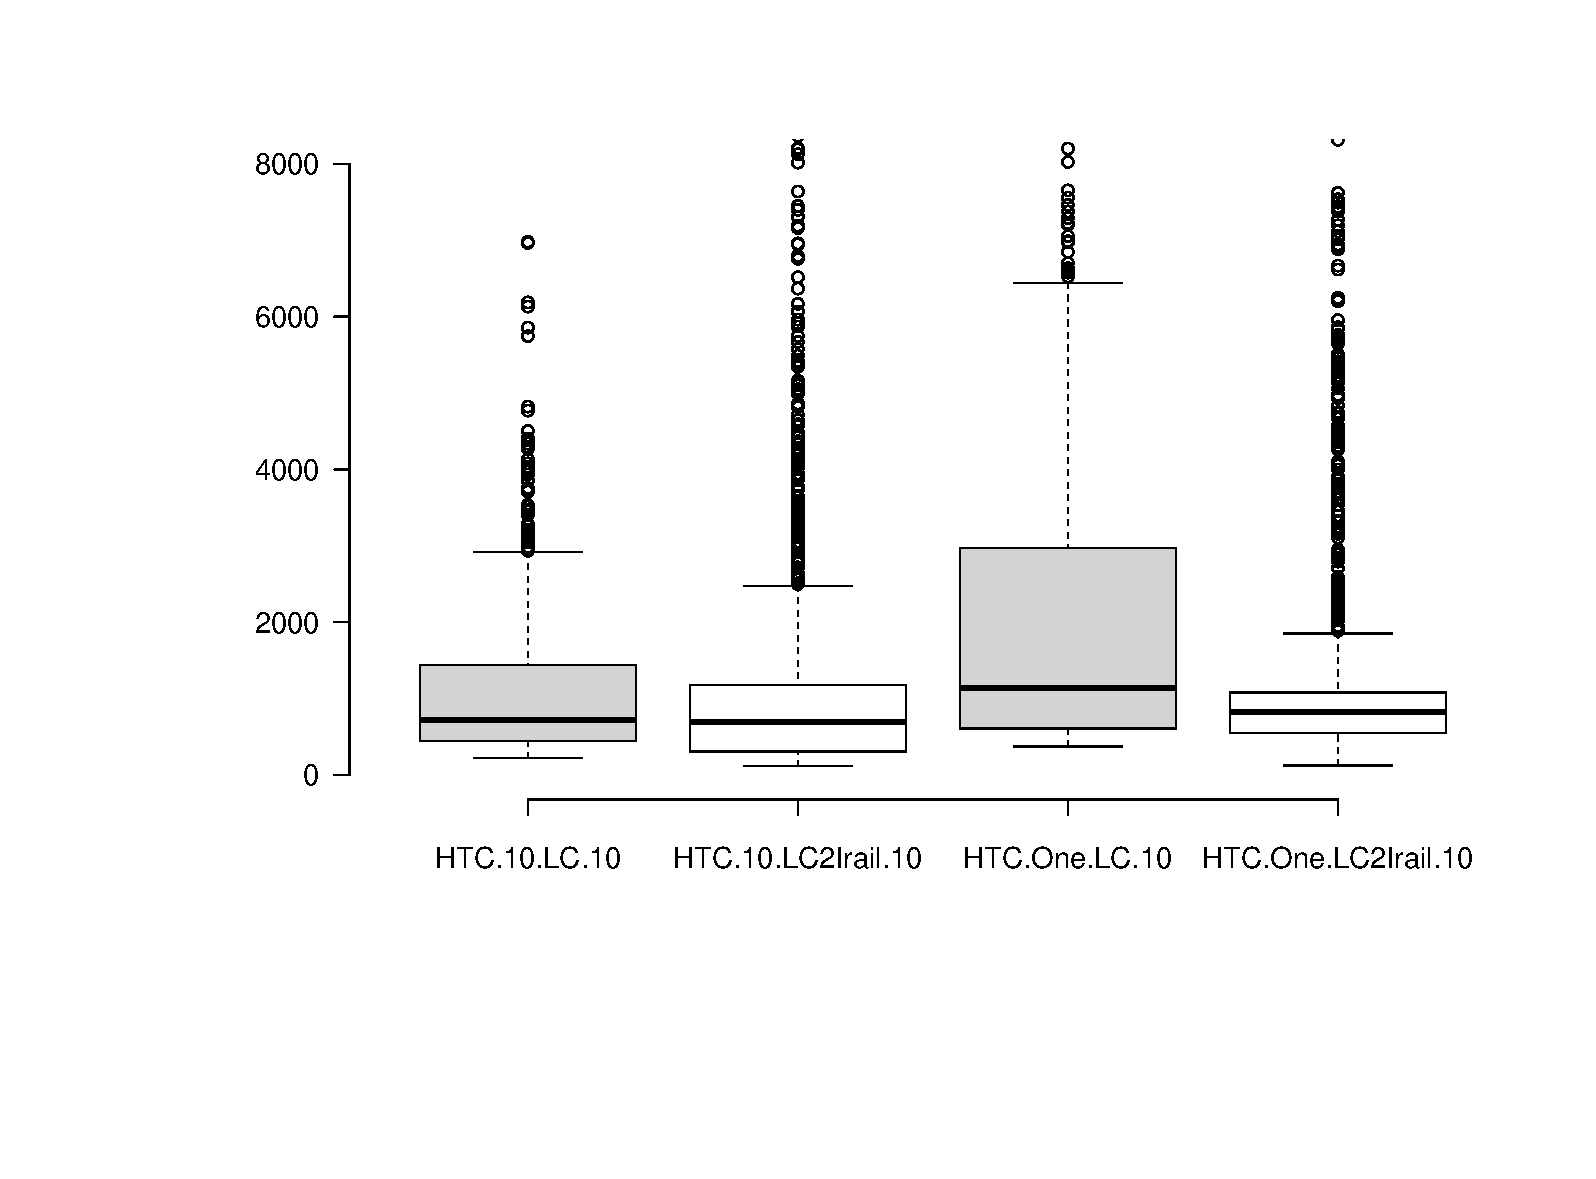
\includegraphics[trim=3cm 4cm 0 0, width=.50\textwidth]{images/boxplot_liveboards_10.eps}
		\caption{\label{fig:liveboardboxplot} The distribution of loading times for liveboard queries with 10 results, using different Web architectures and different devices. While the Linked Connections implementation on the fast device (HTC.10.LC.10) is on par with the LC2Irail performance, is the Linked Connections client performance on the HTC One less consistent.The third percentile lies 1,5 seconds higher compared to the Linked Connections client on the HTC One, meaning this implementation will give a less consistent experience on this device.  }
	\end{center}
\end{figure}

Taking a look at the distributions of the loading times for the tenth results (figure~\ref{fig:liveboardboxplot}) it is confirmed again that \textsc{lc2irail} performs the same on both devices. This contrasts with the Linked Connections client, which has a larger distribution of loading times on the HTC One. While the differences between the median response time of the Linked Connections client on the HTC 10 and \textsc{lc2irail} on both devices cannot be distinguished by end users, there is a clear difference with the median of the Linked Connections implementation on the HTC One.

\begin{figure}[ht]
	\begin{center}
		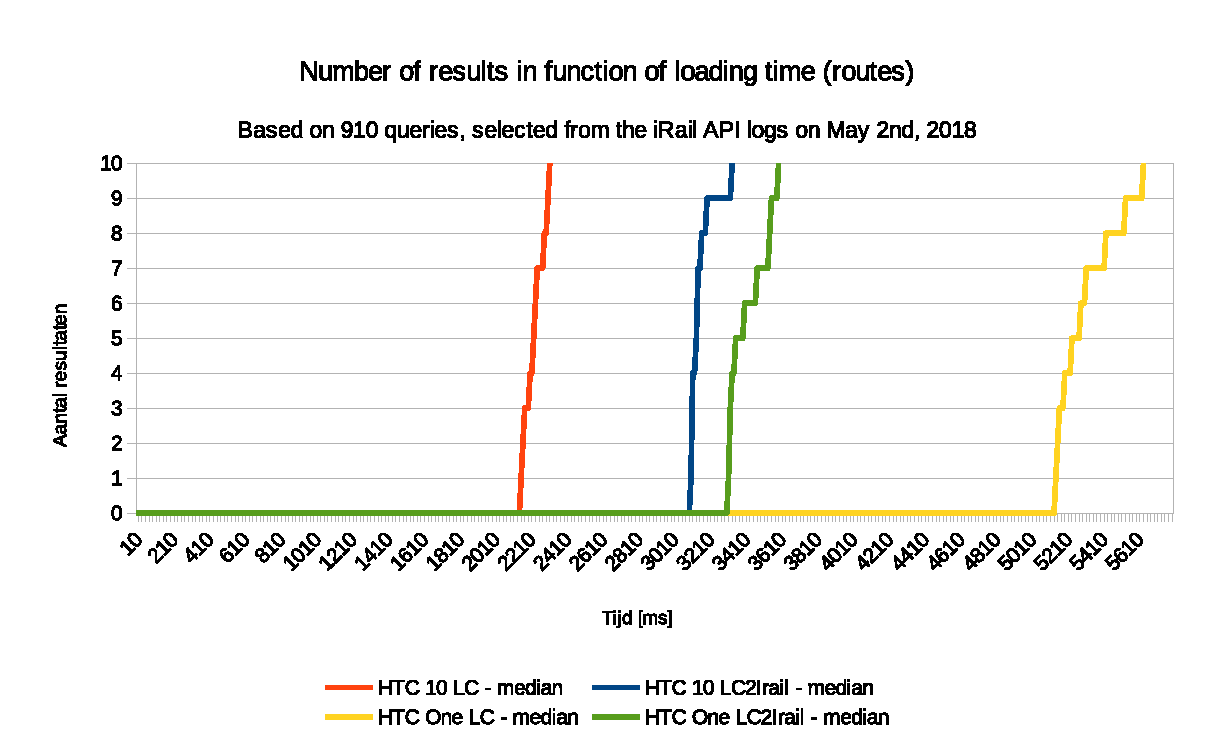
\includegraphics[width=.50\textwidth]{images/dief_routes_average.eps}
		\caption{\label{fig:route} The median performance of loading incremental route results using different Web architectures and different devices shows that for fast devices (HTC-10 LC) client-side filtering gives the first results faster than the server-side implementation (HTC-10 LC2IRAIL). This is opposite to slow devices, where the server-side implementation (HTC One LC2Irail) is 1,8 seconds faster than the client-side implementation (HTC One LC).}
	\end{center}
\end{figure}

When looking at the incremental results for routes (figure~\ref{fig:route}) this difference between devices becomes even more visible. The Linked Connections client loads over 2 times faster on the HTC 10 compared to the HTC One. Due to this the fastest technique depends on the device used. The Linked Connections implementation performs better than \textsc{lc2irail} on the modern HTC 10, but it performs worse than \textsc{lc2irail} on the HTC One. \textsc{lc2irail} performs about the same on both devices, which it also did for liveboards. Calculating routes relies heavily on the Connection Scan Algorithm, which makes it even more surprising to see that Linked Connections on the HTC 10 is faster than the \textsc{rpc} approach. This is also a possible explanation for the strong discrepancy between the loading times of the Linked Connections client on both devices, as the slower processor and memory in the HTC One could hinder both the processing of the raw data, and the calculations using the Connection Scan Algorithm. Distributions for routes are shown in figure \ref{fig:routebox}, where it becomes even more clear that \textsc{lc2irail} sits in between the performance of the Linked Connections client on both devices.

\begin{figure}[ht]
	\begin{center}
		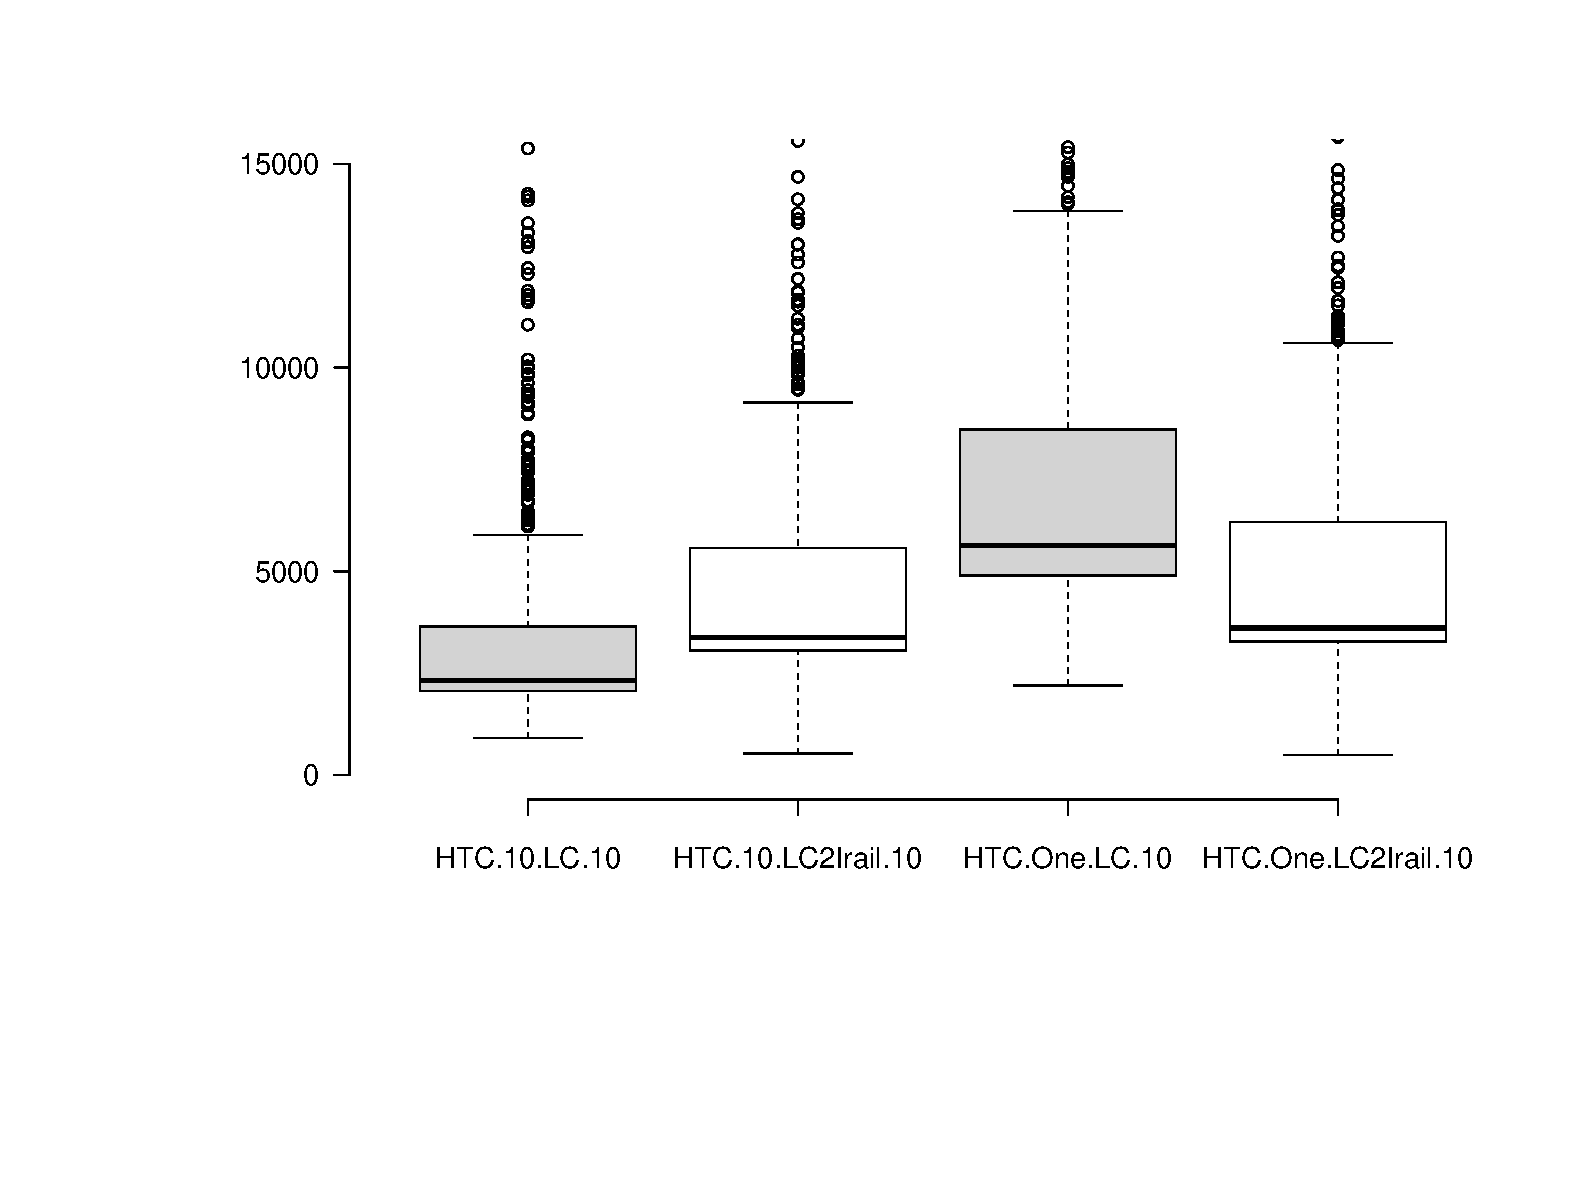
\includegraphics[trim=3cm 4cm 0 0, width=.50\textwidth]{images/boxplot_routes_10.eps}
		\caption{\label{fig:routebox} The distribution of loading times for route planning queries with 10 results, using different Web architectures and different devices. The performance of LC2Irail is similar on both devices (HTC.10.LC2Irail.10 and HTC.One.LC2Irail.10), while the Linked Connections implementation performs better or worse depending on the device. On the fast device (HTC.10.LC.10), the median lies 59\% (3,3s) lower compared to the slower device (HTC.One.LC.10), meaning the tenth result will be loaded more than twice as fast in 50\% of the cases }
	\end{center}
\end{figure}

The performance of \textsc{lc2irail} for Vehicles is special compared to the previous two. Every vehicle trip is considered to be one atomic result, therefore incremental results are not supported for this data type. When looking at the distribution of the loading times (figure~\ref{fig:vehicle}) it becomes clear that vehicles take a long time to load compared to other data structures, even though they are not obtained through complex algorithms. This data type typically needs at least three or four hours of data, which translates in at least six to eight pages, depending on the server configuration. \textsc{lc2irail}, which has quick access to the data, can access pages faster, and has an advantage here. Again, it performs consistently between devices, whereas the Linked Connections implementation needs two times as much time on the HTC One, compared to Linked Connections implementation on the HTC 10.

\begin{figure}[ht]
	\begin{center}
		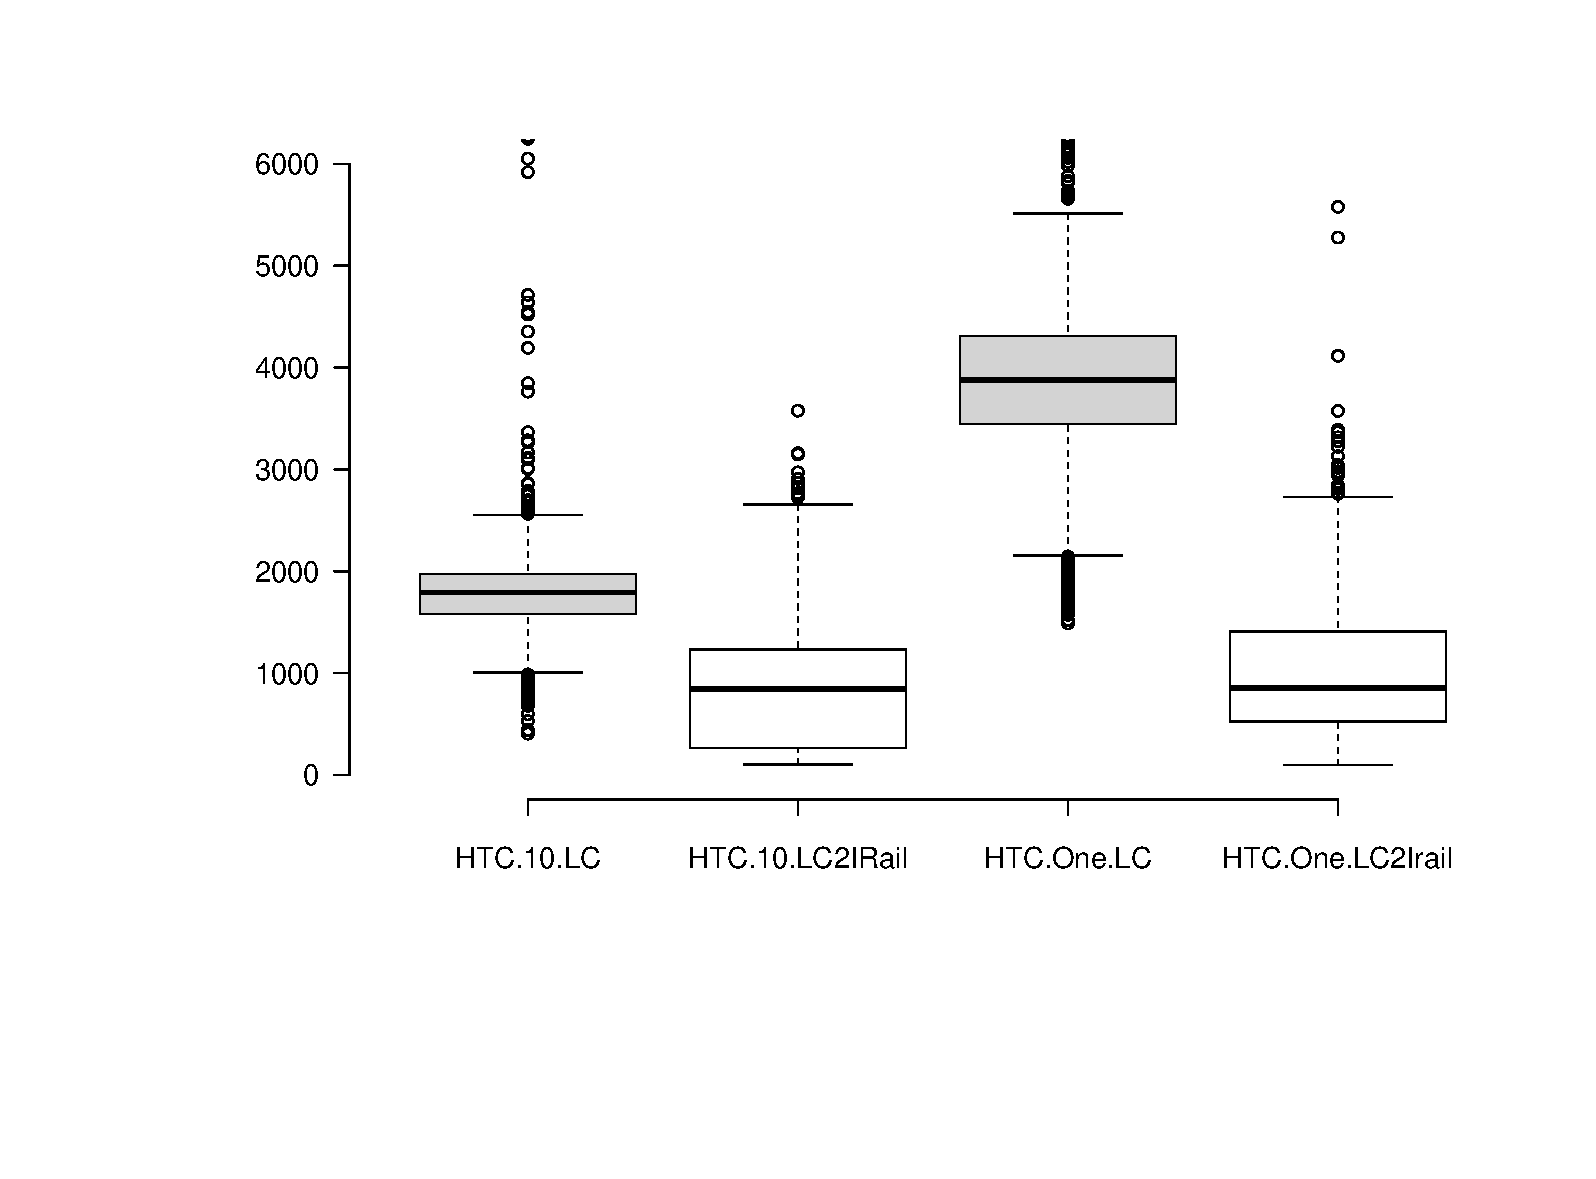
\includegraphics[trim=3cm 4cm 0 0, width=.50\textwidth]{images/boxplot_vehicles.eps}
		\caption{\label{fig:vehicle} The distribution of loading times for vehicle queries, using different Web architectures and different devices. The Linked Connections implementation performs worse on both devices compared to the LC2Irail performance, with the HTC One (HTC.One.LC) taking 2,16 times longer to load the same results compared to the HTC 10 (HTC.10.LC). LC2Irail performs consistent across devices, with only a 7ms difference between the median on both devices (HTC.10.LC2Irail and HTC.One.LC2Irail). }
	\end{center}
\end{figure}

Not only the data type and device affect the performance, but the exact query is of importance too. Calm stations, long routes, or vehicles with a long trip take longer to load compared to busy stations, short routes or vehicles with a short trip. The time to load a number of results is directly related to the timespan in which the results can be
found. When a larger timespan needs to be evaluated, the results will take longer to load.

The measured results seem to match the user experienced performance. This can be seen in figure \ref{fig:choices}. While quite some users still find Linked Connections faster for departures, less people choose Linked Connections for routes, and even less choose Linked Connections for vehicles. However, when users are asked to not only judge by the performance, but to also take additional features like offline access into account, a majority of the users who previously chose for \textsc{lc2irail} changes their mind and chooses Linked Connections. Features like incremental results don’t seem to improve the user-perceived performance – users keep waiting for all results to load before they start processing the results.

\begin{figure}[ht]
	\begin{center}
		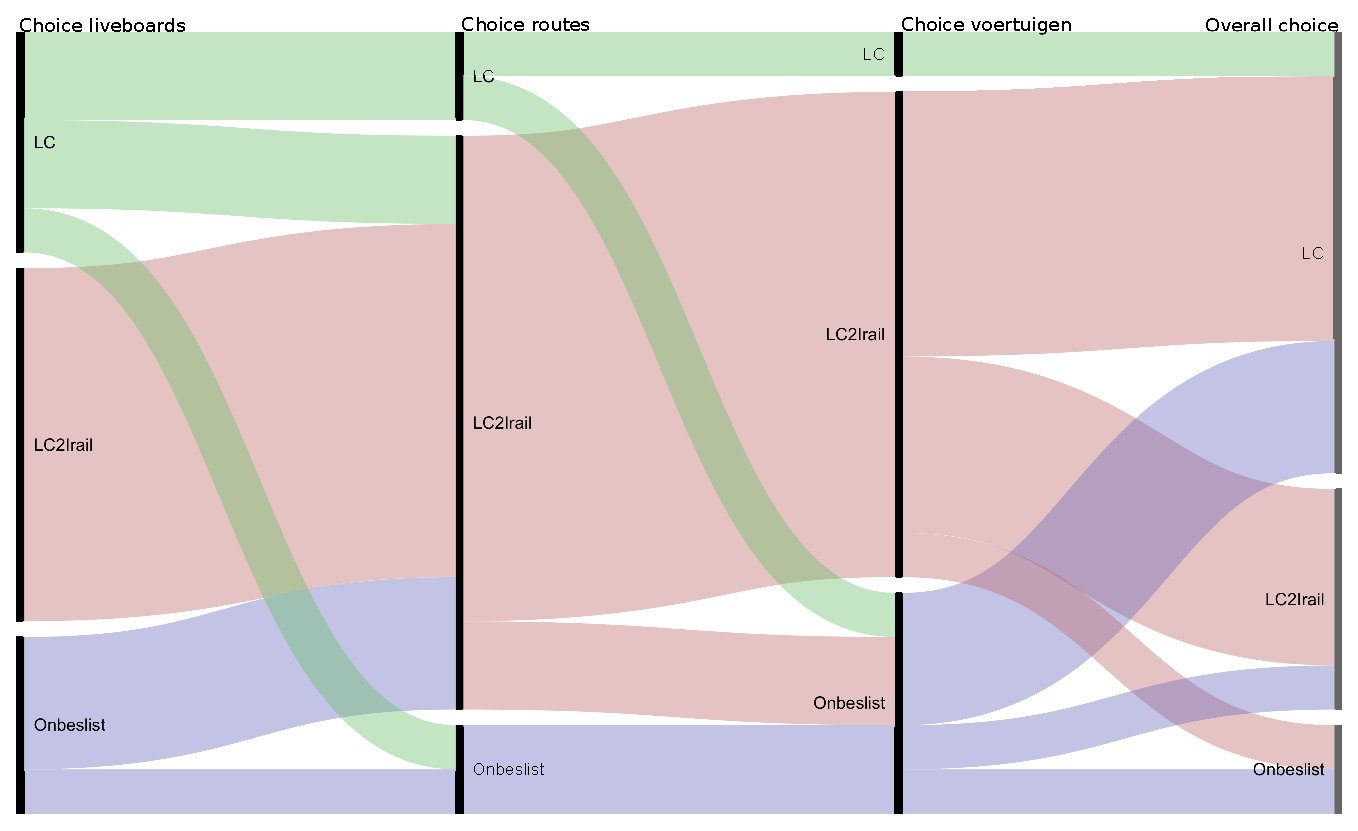
\includegraphics[width=.40\textwidth]{images/alluvial_user_choice_en.eps}
		\caption{\label{fig:choices} The choices users make when asked to pick an implementation based on speed, and when they are asked to make a final decision based on speed and (off-line) functionality. For liveboards, routes and vehicles respectively 29\%, 12\% and 6\% of the testers experience Linked Connections as faster, while 47\%, 76\% and 65\% the users experience LC2Irail faster. Taking off-line access into account, 59\% of the testers picks the Linked Connections implementation as their favourite.  }
	\end{center}
\end{figure}


\section{Discussion}
\textsc{lc2irail} is an ideal reference \textsc{api}. The performance is consistent across devices, and users are overwhelmingly positive over the performance. Consistent good performance, with a small spread of the user-perceived performance, is the goal of every application. Linked Connections seems unable to offer this. The user perceived performance depends heavily on the used device, the type of data which was requested, and on the exact query. Both measured performance and user-perceived performance are spread out, ranging from slower than \textsc{lc2irail} to faster than \textsc{lc2irail}, and from perceived quite slow to perceived extremely fast. It seems there is definitely potential in this technique, but heavy resource requirements are holding it back on older devices.

The difference between both Linked Connections implementations is an extremely important indicator. This difference shows that the performance of Linked Connections
does not only depend on the device, data type and query, but also on the details of the implementation. When the parsing of both implementations is traced, the implementation based on \emph{LoganSquare} is about two times slower than the original implementation, requiring 200 milliseconds to parse a single Linked Connections page, compared to 100 milliseconds when using the \emph{org.json} parser. This is opposite to both benchmarks and user-perceived performance. The key to this mystery is found in the Garbage Collection (\textsc{gc}), ran by the Android Java Virtual Machine (\textsc{jvm}). The first implementation which uses the \emph{org.json} parser creates more String objects than the second implementation based on \emph{LoganSquare}. As String objects are immutable, creating too much of them or modifying them too much will trigger garbage collection, in which case the entire application is frozen as unreferenced objects are removed from the memory. Even further, the \textsc{jvm} garbage collection threshold depends on the heap size, which is configured by the device manufacturer and correlates with the available \textsc{ram} and screen properties. This
means older or cheaper devices are penalized twice: slower hardware means Linked Connections algorithms and \textsc{gc} take more time, while \textsc{gc} will be needed more often as the device has less memory. As a result, \emph{LoganSquare} can be up to 8 times faster than \emph{org.json} for large payloads.

Knowing now the importance of an efficient implementation on all levels, it is possible to reimplement the Linked Connections client while removing or reducing the usage of
Strings. This might lead to further performance improvements, potentially bringing the performance on older or cheaper devices up to par with performance on more powerful devices. Still, this forms a disadvantage for Linked Connections. Developers looking to implement this might not have the necessary (background) knowledge to optimize
their implementation this thorough, or they might not have the time. This could form a barrier for adoption.

Another important curiosity is the U-turn most people made when asked to choose their favourite implementation, based on everything, including speed and offline access.
While more and more people lean towards \textsc{lc2irail} depending on the endpoint, as can be seen in figure 6, off-line access seems to convince over half of the people picking \textsc{lc2irail} to switch to Linked Connections. This can be explained by the general discontent regarding mobile network coverage while travelling by train, and people not having access to mobile data, or being afraid of using too much.

Parameters like data usage depend heavily on the implementation. Various optimizations are possible to reduce this, with off-line access reducing this to zero.

A last important note is the performance after mass adoption. While the \textsc{rpc} \textsc{api} will suffer from reduced performance under high load, Linked Connections provides better performance as load increases. This means the Linked Connections results will only improve, while the performance of the \textsc{rpc} \textsc{api} can only decline.

\section{Conclusion}
While the reference \textsc{rpc} \textsc{api} provides excellent results, Linked Connections offers a wide range of performances depending on various factors, sometimes performing better than this reference \textsc{api}, but in more than 50\% of the cases performing the same or worse. Users consistently perceive Linked Connections as slower, with only some outliers experiencing it faster. Performance heavily depends on the search, implementation and the users’ device. This is a bad trait for an application, as the goal is to present a consistent experience across all devices.

The client-side Android route planning implementation can be improved by paying attention to implementation details such as the performance of used libraries and the use of String objects. Resulting from this research, we see evidence that only a Paged Collection of connections is not sufficient to provide for the basic functionalities of a route planning applications. For the vehicle overview for instance, we suggest adding a mandatory feature to the Linked Connections specification to publish indices on which trips are described in each page, or to allow clients to filter on a trip id. This reduces the overhead of retrieving pages without useful data.

Reducing this network traffic could also be achieved by running the algorithms on cached data first, after which the used pages could be retrieved from the server in order to obtain real-time information. These results based on the cached data could be shown while real-time data is loaded from the server, after which the real-time data could be appended to the first results.

The performance of the route planning algorithm can be further optimized by first applying the Earliest Arrival Time algorithm, which will cache the required pages and determine the starting point where the Connection Scan Algorithm should start iterating over the pages. Search performance could also be improved by pre-loading data when it is highly likely the user will make a search. In this case it is no longer needed to retrieve the pages the moment the user confirms the search.

Keeping recently used pages in memory will speed up the loading of results after the first pages has been downloaded, as it is likely that the next search will require data from the same page as the previous page. In reality, this might not be feasible due to constraints on the available memory. All performance improvements should take the device properties into account, as a device with limited \textsc{ram} might be better off using a cache in the flash memory.

\nocite{*}
\bibliographystyle{phdsymp}
%%%%%\bibliography{bib-file} % commented if *.bbl file included, as
%%%%%see below


%%%%%%%%%%%%%%%%% BIBLIOGRAPHY IN THE LaTeX file !!!!! %%%%%%%%%%%%%%%%%%%%%%%%
%% This is nothing else than the phdsymp_sample2e.bbl file that you would%%
%% obtain with BibTeX: you do not need to send around the *.bbl file  
%%
%%---------------------------------------------------------------------------%%
%
\begin{thebibliography}{1}
\bibitem{colpaert17}
Pieter Colpaert,
\newblock {\em Publishing transport data for maximum reuse},
\newblock Ph.D. dissertation, Ghent University, 2017. [Online]. Available: https://phd.pietercolpaert.be

\bibitem{fielding99}
R. T. Fielding and R. N. Taylor, 
\newblock {\em Principled design of the modern web architecture},
\newblock 1999. [Online]. Available: https://www.ics.uci.edu/~fielding/pubs/fse99\_webarch.pdf

\bibitem{avila11}
J. A. Bargas-Avila and K. Hornbæk, 
\newblock {\em Old wine in new bottles or novel challenges: A critical analysis of empirical studies of user experience,”},
in Proceedings of the SIGCHI Conference on Human Factors in Computing Systems, ser. CHI ’11. New York, NY, USA: ACM, 2011, pp. 2689–2698. [Online]. Available: http://www.kasperhornbaek.dk/papers/CHI2011\_UXReview.pdf

\bibitem{verborgh16}
R. Verborgh, M. Vander Sande, O. Hartig, J. Van Herwegen, L. De Vocht, B. De Meester, G. Haesendonck, and P. Colpaert, 
\newblock {\em Triple pattern fragments: a low-cost knowledge graph interface for the web},
\newblock Journal of web semantics, vol. 37-38, pp. 184–206, 2016. [Online]. Available: http://dx.doi.org/10.1016/j.websem.2016.03.003

\bibitem{rpc}
B. J. Nelson, “Remote procedure call,” Ph.D. dissertation, Pittsburgh, PA, USA, 1981.

\bibitem{dijkstra}
E. W. Dijkstra, 
\newblock {\em A note on two problems in connexion with graphs},
\newblock Numer. Math., vol. 1, no. 1, pp. 269–271, Dec. 1959. [Online]. Available: http://dx.doi.org/10.1007/BF01386390

\bibitem{bellmanford}
R. Bellman,
\newblock {\em On a routing problem},
\newblock Quarterly of Applied Mathematics, vol. 16, pp. 87–90, 1958.

\bibitem{csa}
J. Dibbelt, T. Pajor, B. Strasser, and D. Wagner,
\newblock {\em Connection Scan Algorithm},
\newblock CoRR,vol. abs/1703.05997, 2017. [Online]. Available: http://arxiv.org/abs/1703.05997

\end{thebibliography}
%
%%---------------------------------------------------------------------------%%

\end{document}

%%%%%%%%%%%%%%%%%%%%% End of phdsymp_sample2e.tex %%%%%%%%%%%%%%%%%%%%%%%%%%%
